\chapter{An Overview of the Genome Properties Database, InterPro and InterProScan5} \label{genome-properties} 

The architecture and implementation of Micromeda's components, such as Pygenprop and Micromeda-Client, are closely tied to the structure of the Genome Properties database. As mentioned in Section XXX, Micromeda uses Pygenprop to predict the biochemical pathways possessed by an organism. This prediction is done by providing Pygenprop with a copy of the Genome Properties database and the output of running InterProScan5 on the organism's predicted protein sequences. In addition to discussing the structure of the Genome Properties database, this chapter will discuss this pathway prediction process is carried out. Specifically, how InterProScan5 performs domain annotation on an organisms proteins and how the Genome Properties database uses these domains as markers for identifying the presence of specific enzymes that support the existence of pathway steps.

\section{An introduction to Protein Domains and their use as Markers of Enzyme Function}

A protein domain is conserved part of a protein's sequence that carries out a specific function for the protein and is evolutionarily conserved. These domains often generate discrete three-dimensional structures during folding of their parent protein. An enzyme's function is highly correlated with its domain content. For example, all enzymes have an active site (\href{en.wikipedia.org/wiki/Active\_site}{en.wikipedia.org/wiki/Active\_site}), a pocket area on its three-dimensional folded shape, that directly interacts with substrates (see Section \ref{enzymes-and-pathways}). This active site area has a unique sequence of amino acids, a protein domain, that is often uniquely identifiable to a specific enzyme or enzyme family. Often proteins consist of a series of domains that are chained together. For example, a protein that embeds itself within a cell membrane will have a domain associated with this capability \footnote{Proteins that have a specific set of amino acids on parts of their surface become hydrophobic and tend to embedded themselves within cell membranes that are also hydrophobic. Protein sequence patterns associated with this trait are easily recognized by software.} in addition to its catalytic domain. Similar to how different enzymes can be swapped in and out of biochemicals pathways, domains can also be gained and lost from their host proteins overtime and according to evolutionary forces. For example, enzymes that are evolutionarily related may locate differently in cell due to the presence or absence of a membrane associated domain. It is quite common to have some members of a enzyme family cystolic (i.e., free floating within the cell) versus others membrane bound. Thus in some ways an enzymes domain content can be used as marker of both its function and cellular localization.

The Genome Properties database uses combinations of protein domains to identify enzymes that may carry out pathway steps. If these domains are present in the proteins of the organism then a step of a pathway can be considered to be present. The domains used by the Genome Properties database are those catalogued within the InterPro consortium of protein databases.

\section{The InterPro Consortium of Protein Databases}

Similar to how information about biochemical pathways have been catalogued within databases (see Section XXX), information about proteins and protein domains have also been catalogued in databases. Since different types of metabolism are shared across many organisms and the enzymes that carry out each step in this metabolism are highly similar, it is useful to categorize proteins into groups that carry out a single function. Protein databases record the function of these groups of proteins and their domains. These databases also store copies of the sequences of examples of these proteins or domains. In the past many of these protein databases were maintained and operated independently by a variety of different research organisations. However, in the past two decades many of the operators of these databases have banded together to form the the InterPro consortium, which is head by the European Bioinformatics Institute (EBI). As of 2019, the InterPro consortium of protein databases contains fourteen member databases. Examples of such databases include PFAM, TIGRFAM, PANTHER, the Conserved Domain Database (CDD), HAMAP, PRINTS  and many others. In addition to the member databases, the consortium also provides the InterPro database, which is a meta-database that allows for mapping between identical records for same protein or domain families across member databases. Each protein or domain catalogued is given a global InterPro identifier (e.g. IPRXXXX) that is mapped to multiple identifiers within member databases (e.g. PFXXXX or TFXXXX). For the most part, each InterPro protein or domain is only catalogued by a subset of member databases within the consortium.

An import feature of any protein databases is to be able to provide it with novel protein and find the protein's closest match within the database. Such databases perform this operation by performing sequence similarity searches between the novel protein and member proteins. However, because each each record in the InterPro database can represent multiple representative proteins, a method has to be performed that compares the novel proteins to all representative proteins of a specific group. Rather than comparing the novel protein to each within the group, a more efficient way to perform such comparisons is to compare the novel protein to a model, or profile, that represents the sequence diversity (i.e., not all proteins in a family are exactly the same) for each protein or domain group held with the database. Such models are built from alignments of all proteins within a database. These alignments are used to gather regions of shared similarity across members of a family. If the novel protein, when compared to a model, also possesses these regions of high similarity it is more likely that the novel protein is a member of the protein family that the model represents, than if it did not possess these regions. This model-based approach reduces the number of searchers required to find which group that a novel protein belongs to and is highly accurate. Examples of such approaches include Position-Specific Scoring matrices (PSSMs) and hidden Markov models (HMMs).

\begin{figure}[!ht]
  \centering
	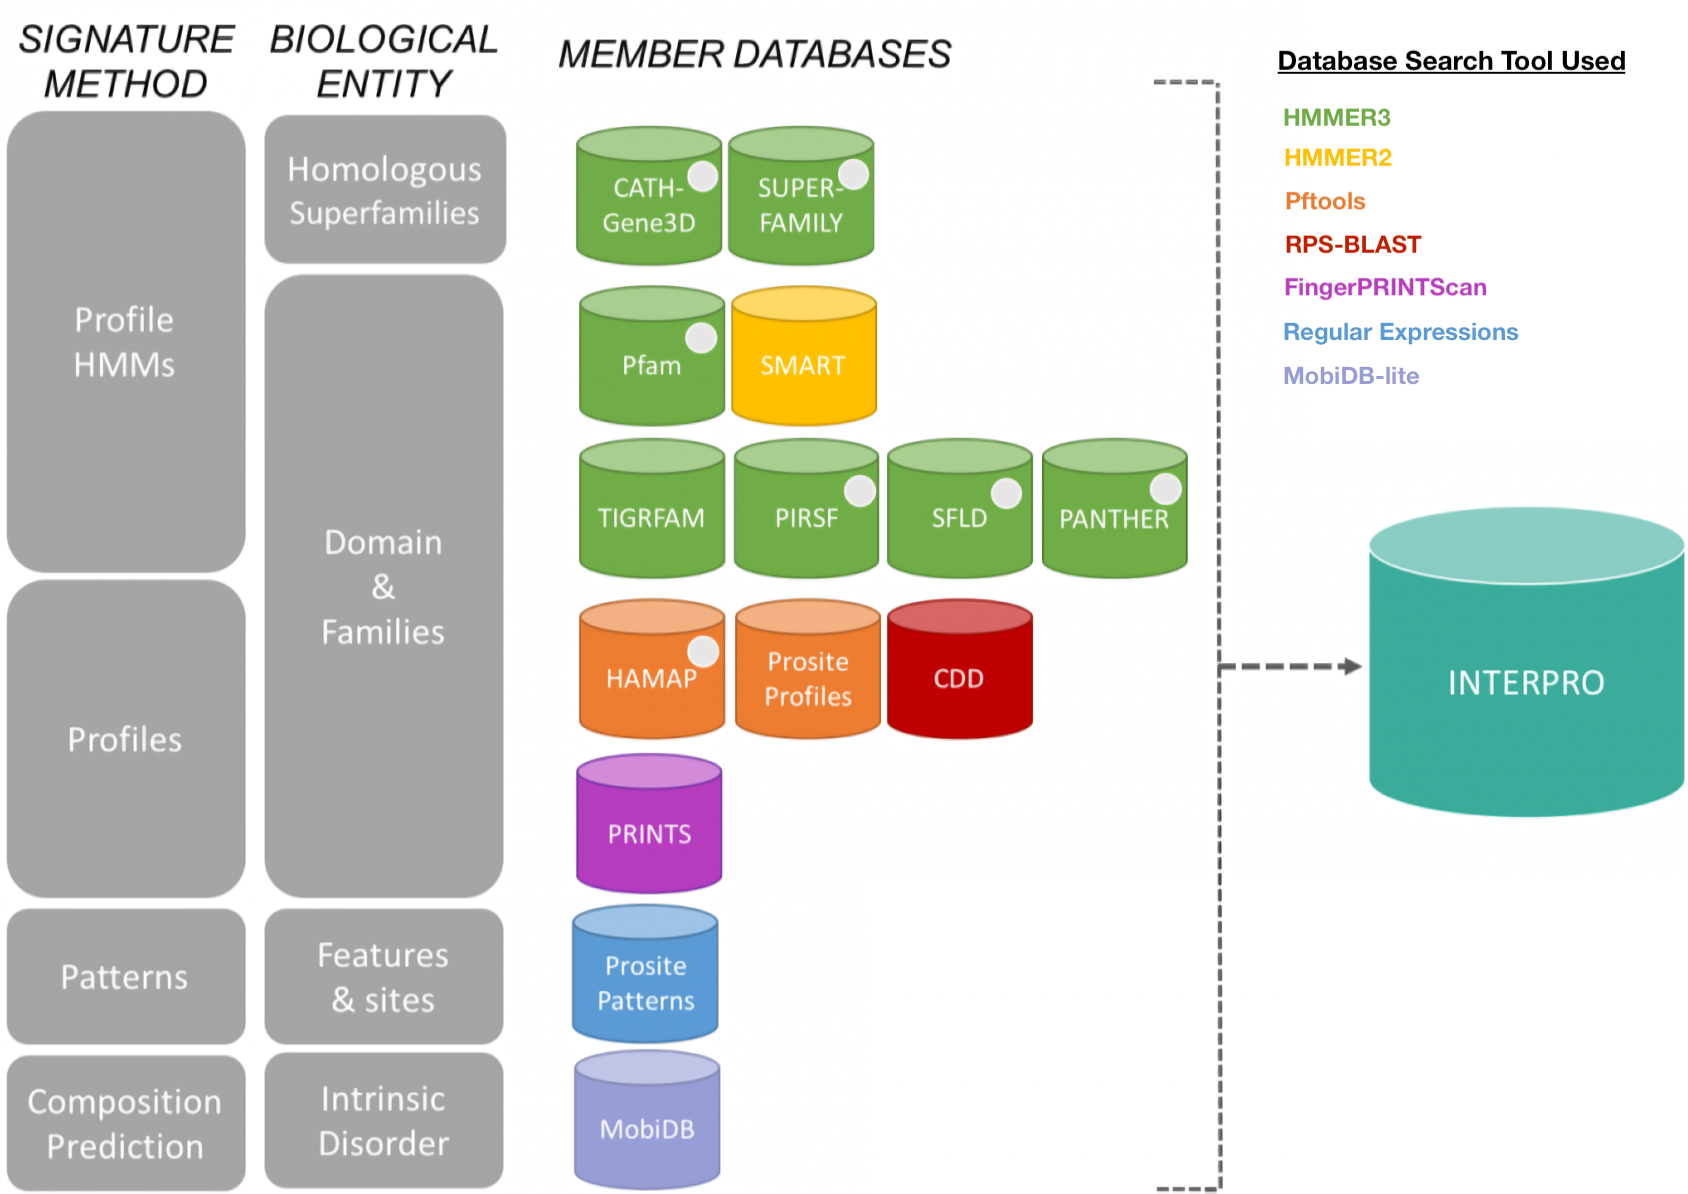
\includegraphics[width=0.90\textwidth]{media/InterPro.png}
	 \caption{The InterPro consortium of protein databases Use A Variety of methods to classify novel protein Sequences. Multiple sequence search softwareS are used for finding motifs in protein sequences of interest.}
	 \label{fig:interpro-databases}
\end{figure}

Because the member databases of the InterPro consortium were developed independently, the methods these use for sequence search also vary. The majority of these use a piece of software called HMMER that can be used to build an HMM model of the sequence of a family of proteins or a domain and then use this model to determine if a novel protein is a member of the family or is highly similar to the domain. The Conserved Domain Database uses pre-calculated PSSMs and PSIBLAST to classify novel proteins. Some of the member databases even use simple techniques such as Regular Expressions (REGEXs) to identify sequences similarity between novel and database proteins. Most of these search techniques return an evaluation of how similar the novel protein is to the database model.

Motifs are discrete patterns in a protein's sequence, that are often associated with the existence of a protein domain. Domain annotation is the process of predicting the placement and function of domains in protein sequences. During the genomic analysis, it is common practice to perform domain annotation on an organism's predicted proteins.

Domain annotations of an organism's proteins are created by finding similarities between motifs in an organism's proteins and previously seen motifs of domains from other proteins found in a protein database. If an organism and database motif are highly similar in protein sequence, they are said to form a match. The quality of this match can be quantified by metrics such as expected value (E-value) score. A match's E-value score captures how likely it is that the match is real given the chance of finding an equivalent match randomly in one of the organism's other proteins. If we determine that a match is of high quality, the motif in the organism's protein can be assigned the same name and function as the original domain motif the protein database. As member databases were eventually folded into the InterPro consortium the InterPro website created a tool that allows users to compare an uploaded protein sequence to the protein families and domains found within member databases. This tool is called InterProScan,.

\section{InterProScan}

One tool for performing domain annotation of an organism's proteins is InterProScan, which predicts both the type and placement of domains in an organism's proteins and also provides supporting match information to justify its predictions. This supporting information includes E-value scores for matches and predicted domain start and stop points on the annotated protein. InterProScan takes a FASTA file \cite{pearson19905} containing an organism's predicted proteins (as would be created by Prodigal) as input and writes domain annotations and match data to tab-separated value (TSV) files.

\section{The Genome Properties Database}

\subsection{The Structure of the Genome Properties database}

\subsection{Overview of the Genome Properties Flat File Database and Associated File Formats} \label{Genome-Properties-Files} \label{genome-properties-files}

The Genome Properties database (as of version 2.0) consists of a series of flat files that are hosted inside a Github repository (see \href{github.com/ebi-pf-team/genome-properties}{github.com/ebi-pf-team/genome-properties}). Information about individual properties is stored in the repository's \textbf{data} folder, and within this folder, each property is assigned a second internal folder containing three files: 
\begin{itemize}
\item A \textbf{DESC} file, that contains information about the property
\item A \textbf{status} file that contains information onto whether the property is public or has been manually curated
\item A \textbf{FASTA} \cite{pearson19905} file containing representative protein sequences that carry out the steps a the property
\end{itemize}
The \textbf{data} folder contains information about both public and non-public genome properties. 

In addition to the per-property folders, there is also a Genome Properties release file located in the \textbf{flatfiles} folder of the repository that also contains Genome Properties information. Specifically, this file, called \textbf{genomeProperties.txt}, is a concatenation of all the \textbf{DESC} files of all public properties. This file is created with each new release of the Genome Properties database on Github. Below is simplified a folder structure for the Genome Properties Github repository.

\begin{verbatim}
├── code/ - # The Genome Properties Perl library.
├── data/ - # Data about both public and private properties
│ ├── GenProp0001/
│ │ ├── DESC - # Detailed property information
│ │ ├── FASTA - # Sequences of proteins that carry out steps
│ │ └── status - # Public and manual curation status
│ └── GenProp0002/
│  ├── DESC
│  ├── FASTA
│  └── status
└── flatfiles/
 └── genomeProperties.txt
\end{verbatim}

The Genome Properties database parser is capable of parsing both single \textbf{DESC} files of individual properties and the concatenated \textbf{genomeProperties.txt} release file. The format of \textbf{DESC} files is very similar to the Stockholm sequence alignment format used by both the Pfam and Rfam databases \cite{bateman2004pfam, griffiths2003rfam}. Like these file types, \textbf{DESC} files consist of a series of key-value pairs. Because these files use different keys than Stockholm, a custom parser had to be developed. It is of note that the Genome Properties database format wraps every eighty characters. Thus, some key types that contain long sentences are repeated for multiple lines and the parser must unwrap these lines to prevent parsing errors. Below is an example \textbf{DESC} file and a summary of key types can be found in Table \ref{table:property-file-keys}.

\begin{verbatim}
AC GenProp0145
DE Histidine degradation to glutamate
TP PATHWAY
AU Haft DH
TH 2
RN [1]
RM 2203753
RT Nucleotide sequence of the gene encoding the repressor for the
RT histidine utilization genes of Pseudomonas putida.
RA Allison SL, Phillips AT;
RL J Bacteriol. 1990;172:5470-5476.
RN [2]
RM 25559274
RT Structure of N-formimino-L-glutamate iminohydrolase from Pseudomonas 
RT aeruginosa.
RA Fedorov AA, Martí-Arbona R, Nemmara VV, Hitchcock D, Fedorov EV, Almo SC, 
RA Raushel FM;
RL Biochemistry. 2015;54(3):890-7.
DC Histidine Catabolism
DR IUBMB; AminoAcid; His3;
DC Histidine Metabolism
DR KEGG; map00340;
DC L-histidine degradation II
DR MetaCyc; PWY-5028;
CC This pathway is involved in histidine utilization system (hut). HutP is
CC the first gene in the hut operon encoding the hutHUIG operator and a
CC positive regulator of the operon, activated allostatically in the
CC presence of L-histidine. HutC represses histidine utilization by binding 
CC the regulatory sites for hutHUIG and hutF [1]. There are multiple
CC variations in the histidine degradation pathway, including two possible 
CC routes for the first step (either via histidine transaminase, or as in 
CC this pathway, via histidine ammonia-lyase/histidase). L-histidine is 
CC first converted to urocanate by hutH (histidine ammonia-lyase), that is 
CC then converted to 4-imidazolone-5-propionate by hutU (urocanate 
CC hydratase), and finally hydrolysed to N-formimino-L-glutamate by hutI 
CC (imidazolonepropionate amidohydrolase). From here there are three 
CC potential paths to glutamate. This property refers to the two-step 
CC process found in some bacteria where N-formimino-L-glutamate is first 
CC converted to N-formyl-l-glutamate by hutF (formimidoylglutamate 
CC deiminase) and then hydrolyzed to L-glutamate by hutG 
CC (N-formyl-l-glutamate deformylase)[2].
** Evidence for steps 4 and 5 is the same.
--
SN 1
ID Histidine ammonia-lyase (hutH)
DN Histidine ammonia-lyase/hutH (EC 4.3.1.3)
RQ 1
EV IPR005921; TIGR01225; sufficient;
TG GO:0006548;
--
SN 2
ID Urocanate hydratase (hutU)
DN Urocanate hydratase/hutU (EC 4.2.1.49)
RQ 1
EV IPR023637; TIGR01228; sufficient;
TG GO:0006548;
--
SN 3
ID Imidazolonepropionase (hutI)
DN Imidazolonepropionase/hutI (EC 3.5.2.7)
RQ 1
EV IPR005920; TIGR01224; sufficient;
TG GO:0006548;
--
SN 4
ID Formimidoylglutamate deiminase/formiminoglutamase/glu-formyltransferase
DN Formimidoylglutamate deiminase/hutF (EC 3.5.3.13)
RQ 1
EV IPR005923; TIGR01227; sufficient;
TG GO:0006548;
EV IPR010252; TIGR02022; sufficient;
TG GO:0006548;
EV IPR004227; TIGR02024; sufficient;
TG GO:0006548;
--
SN 5
ID Formylglutamate deformylase/formiminoglutamase/glu-formyltransferase
DN N-formylglutamate deformylase/hutG (EC 3.5.1.68)
RQ 1
EV IPR005923; TIGR01227; sufficient;
TG GO:0006548;
EV IPR010247; TIGR02017; sufficient;
TG GO:0006548;
EV IPR004227; TIGR02024; sufficient;
TG GO:0006548;
--
SN 6
ID Histidine utilization repressor (hutC)
DN Histidine utilization repressor/hutC
RQ 0
EV IPR010248; TIGR02018; sufficient;
//
\end{verbatim}

% Please add the following required packages to your document preamble:
% \usepackage{longtable}
% Note: It may be necessary to compile the document several times to get a multi-page table to line up properly
\begin{longtable}{|l|l|}
\caption{Genome Properties \textbf{DESC} files use a variety of keys to provide information about a single property. The below table is copied from the Genome Properties database \href{genome-properties.readthedocs.io/en/latest/flatfile.html\#desc-file}{documentation}.}
\label{table:property-file-keys}\\
\hline
\textbf{Key} & \textbf{Information Type} \\ \hline
\endfirsthead
%
\multicolumn{2}{c}%
{{\bfseries Table \thetable\ continued from previous page}} \\
\hline
\textbf{Key} & \textbf{Information Type} \\ \hline
\endhead
%
AC & Accession ID \\ \hline
DE & Description/name of Genome Property \\ \hline
TP & Type \\ \hline
AU & Author \\ \hline
TH & Threshold \\ \hline
RN & Reference number \\ \hline
RM & PMID of reference \\ \hline
RT & Reference title \\ \hline
RA & Reference author \\ \hline
RL & Reference citation \\ \hline
DC & Database title \\ \hline
DR & Database link \\ \hline
PN & Parent accession ID \\ \hline
CC & Property description \\ \hline
** & Private notes \\ \hline
– & Separator \\ \hline
SN & Step number \\ \hline
ID & Step ID \\ \hline
DN & Step display name (includes EC number if available) \\ \hline
RQ & Required step \\ \hline
EV & Evidence (includes whether sufficient) \\ \hline
TG & Gene Ontology (GO) ID \\ \hline
// & End \\ \hline
\end{longtable}

\section{Summary}

Data summary doe.